%%
%  ******************************************************************************
%  * #file    Szablon_raportu_EN_Latex.tex
%  * #author  Adrian Wójcik   adrian.wojcik(at)put.poznan.pl
%  *          
%  * #commit  Patryk Kościk   koscikpatryk(at)gmail.com
%  *          Modified the template for Projekt przejsciowy purposes          
%  *          
%  * #version 1.0
%  * #date    09-Mar-2022
%  * #brief   PROJPRZEJ
%  *
%  ******************************************************************************
%%  
\documentclass[11pt, a4paper]{article}

\usepackage{setup}

% Wypełnijcie te dyrektywy zgodnie z waszym tematem
% \lab      -> NAZWA CZUJNIKA, np.: 'DHT22'
% \comment  -> Króciutki opis co to, np.: 'Cyfrowy budżetowy czujnik temperatury'
%
\lab{Czujnik odległości}
\comment{czujnik HY-SRF05}
\author{Adam Rewekant}

% Absolutny zakaz dotykania tego tutaj bo jak dotkiecie to coś jebnie
\university{Politechnika Poznańska}
\faculty{Wydział Automatyki, Robotyki i Elektrotechniki}
\institute{Instytut Robotyki i Inteligencji Maszynowej}
\department{Zakład Sterowania i Elektroniki Przemysłowej}
\addbibresource{bib/elem.bib}
\nocite{*}

%%
%
% Początek dokumentu
%
%%
\begin{document}

%% Strona tytułowa %%
\mainpage{{fig/element/fig6}}

\newpage
\section*{Opis elementu} \addcontentsline{toc}{section}{Wstęp}
Moduł czujnika odległości HY-SRF05 posiada nadajnik i odbiornik, które są przetwornikami ultradźwiękowe piezoelektrycznymi oraz moduł przetwarzania sygnałów, generujący impuls w momencie odbioru wiązki powracającej do czujnika po odbiciu od przeszkody.



\vspace{0.5cm}
\begin{figure}[h]
\centering
\begin{subfigure}{.5\textwidth}
  \centering
  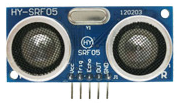
\includegraphics[width=.5\linewidth]{fig/element/fig2.png}
  \caption{HY-SRF05 \cite{fot2}}
  \label{fig:sub1}
\end{subfigure}%
\begin{subfigure}{.5\textwidth}
  \centering
  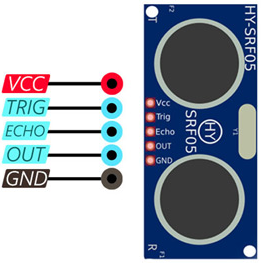
\includegraphics[width=.5\linewidth]{fig/element/fig1.png}
  \caption{HY-SRF05 \cite{fot2}}
  \label{fig:sub2}
\end{subfigure}
\caption{Przykładowe zdjęcia czujnika.}
\label{fig:test}
\end{figure}
\vspace{0.5cm}

Wejście TRIG, służy mikrokontrolerowi jako rozpoczęcie nadawania wiązki ultradźwięków, uruchamiając jednocześnie odliczanie czasu do wykrycia impulsu powrotnego.


\vspace{0.5cm}
\begin{figure}[h]
\centering
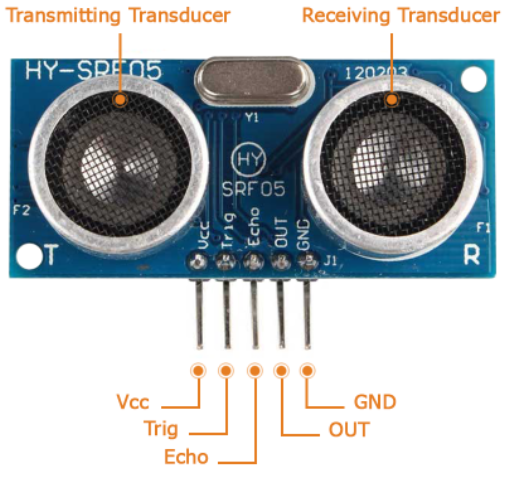
\includegraphics[width=.65\linewidth]{fig/element/fig3.png}
\caption{Budowa czujnika.\cite{fot3}}
\label{fig:test}
\end{figure}
\vspace{0.5cm}

\newpage
\section{Użycie czujnika}

\vspace{0.5cm}
\begin{figure}[h!]
    \centering
    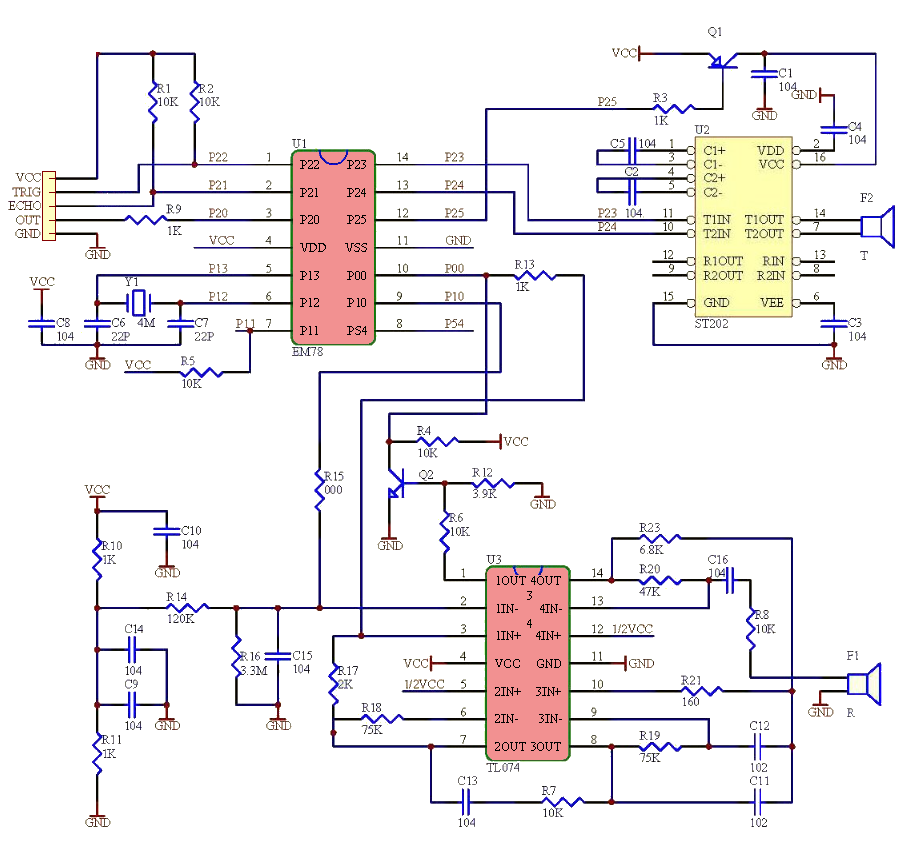
\includegraphics[width=\linewidth]{fig/element/SRFkicad.png}
    \caption{Połaczenie elektryczne}
    \label{fig:my_label}
\end{figure}
\vspace{0.5cm}

Dobrym zastosowaniem dla modułu czujnika odległości jest budowanie map 2D pomieszczenia oraz wykrywanie przeszkód w otoczeniu np. robota autonomicznego. 

\newpage
\clearpage
\section{Prezentacja działania układu}

\vspace{0.5cm}
\begin{figure}[h!]
    \centering
    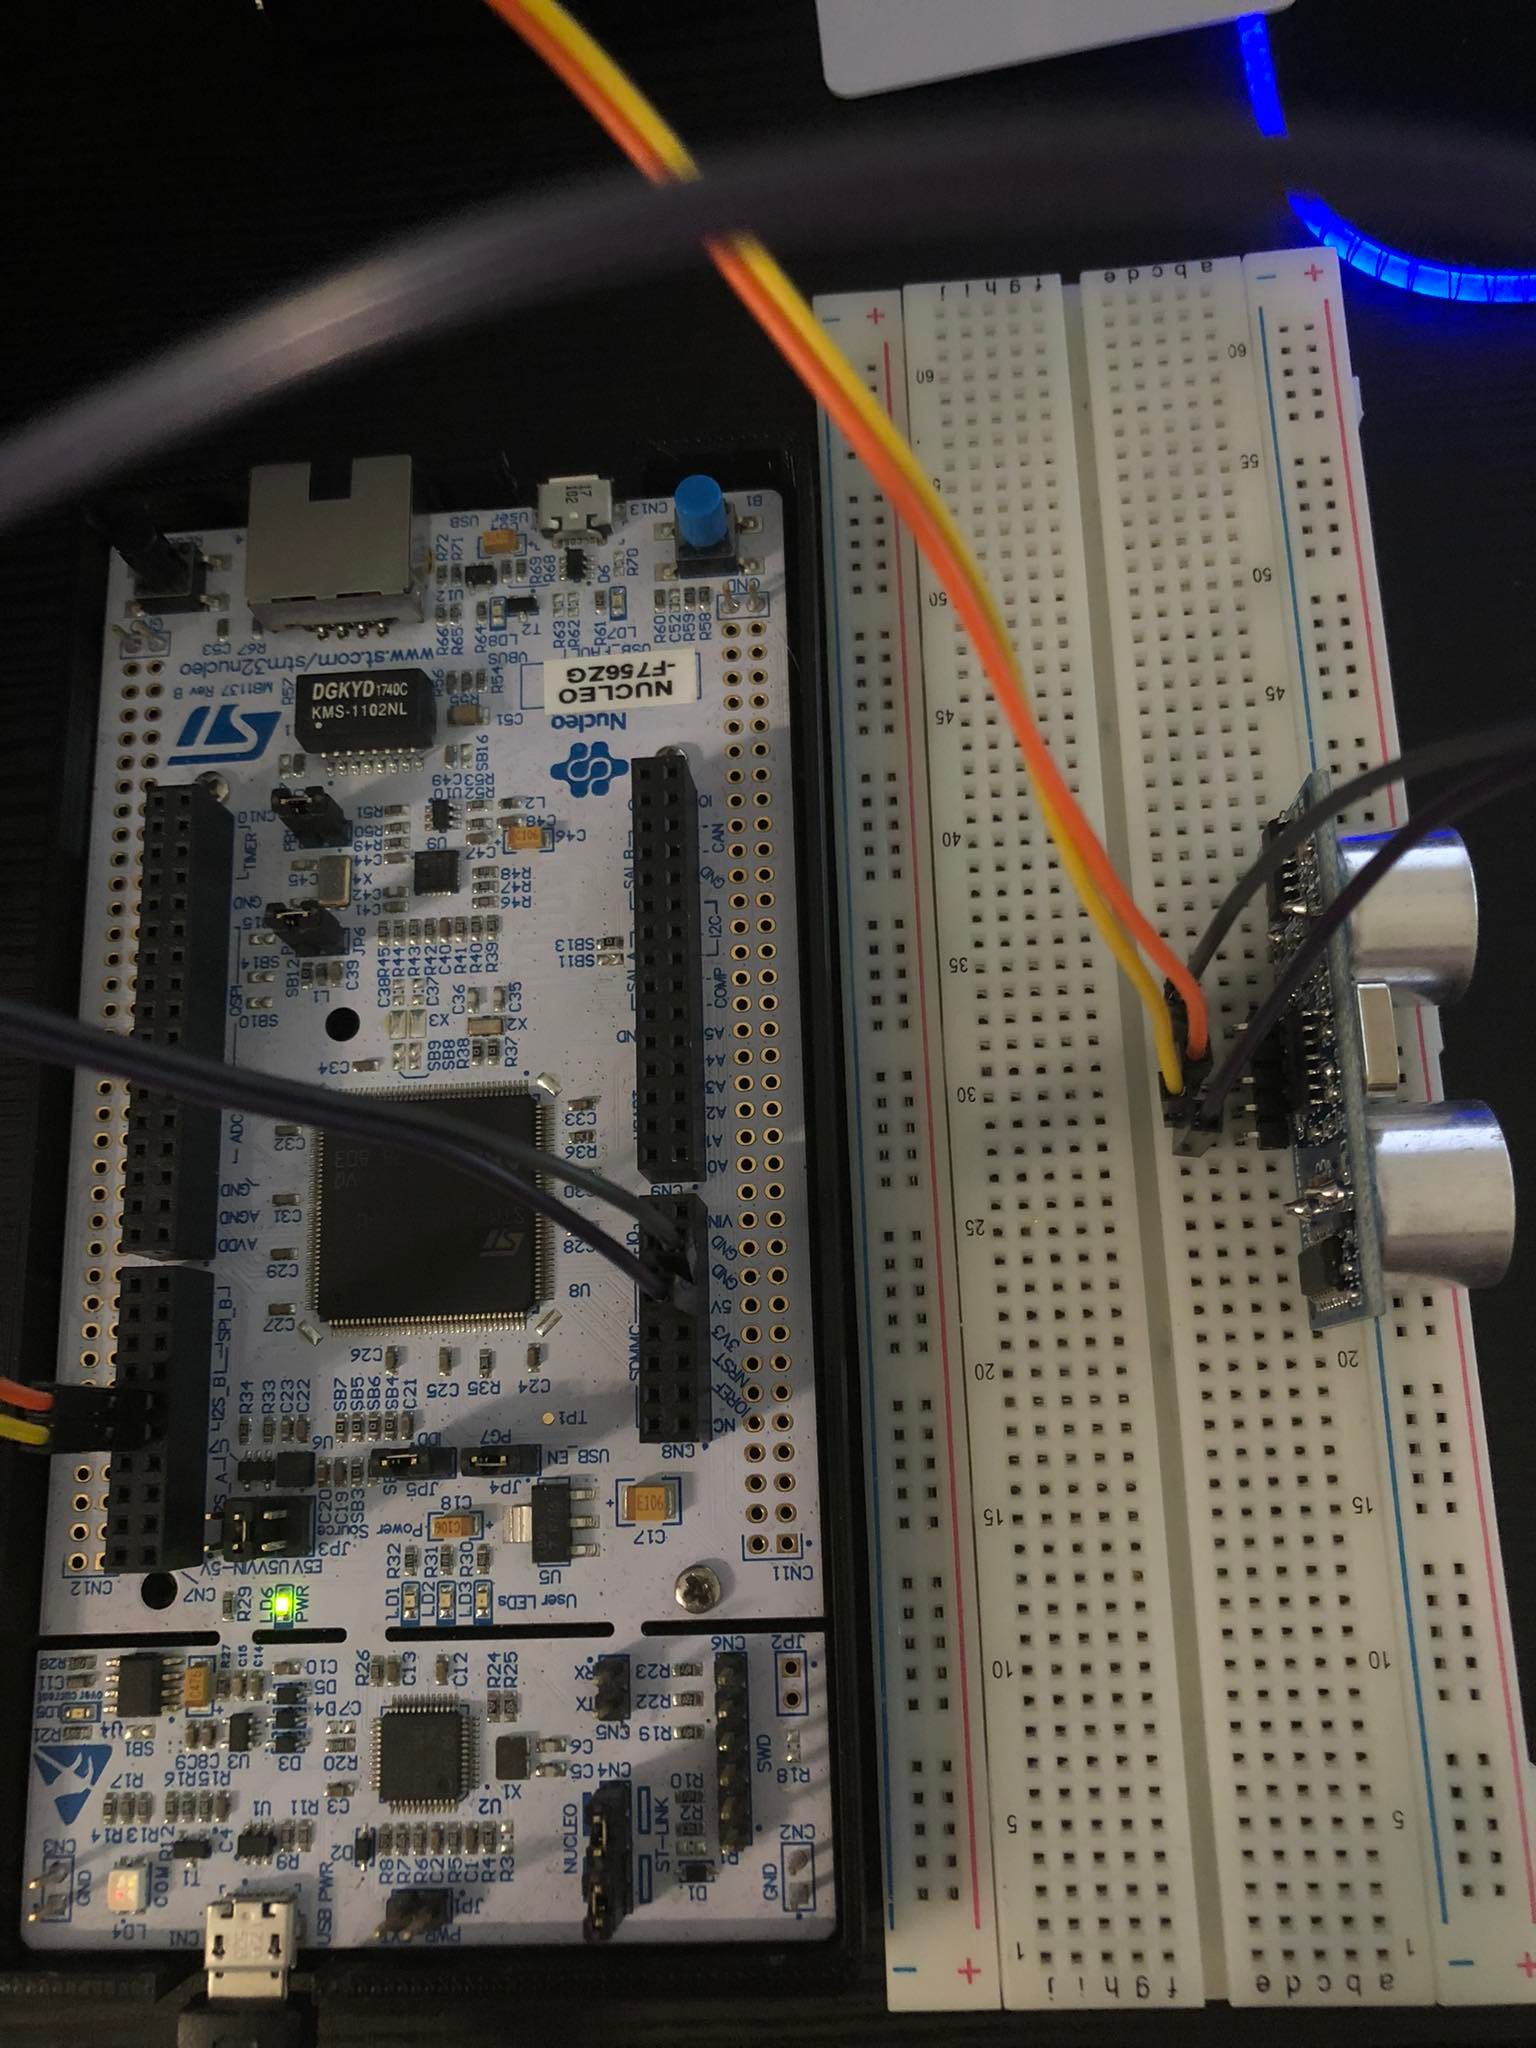
\includegraphics[width=.9\textwidth]{fig/element/foto1.png}
    \caption{Zdjęcie układu.}
    \label{fig:my_label}
\end{figure}

\vspace{0.5cm}
\begin{figure}[h!]
    \centering
    \includegraphics[width=\textwidth]{fig/element/dis5z.png}
    \caption{Pomiar z odległości 5cm.}
    \label{fig:my_label}
\end{figure}

\vspace{0.5cm}
\begin{figure}[h!]
    \centering
    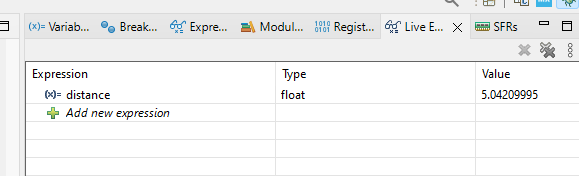
\includegraphics[width=\textwidth]{fig/element/dis5.png}
    \caption{Wynik dla odległości 5cm.}
    \label{fig:my_label}
\end{figure}

\newpage

\vspace{0.5cm}
\begin{figure}[h!]
    \centering
    \includegraphics[width=\textwidth]{fig/element/dis7z.png}
    \caption{Pomiar z odległości 7cm.}
    \label{fig:my_label}
\end{figure}

\vspace{0.5cm}
\begin{figure}[h!]
    \centering
    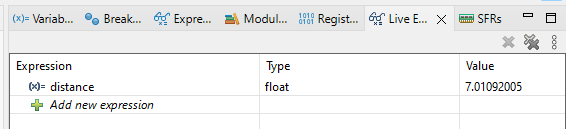
\includegraphics[width=\textwidth]{fig/element/dis7.png}
    \caption{Wynik dla odległości 7cm.}
    \label{fig:my_label}
\end{figure}

\newpage

\vspace{0.5cm}
\begin{figure}[h!]
    \centering
    \includegraphics[width=.9\textwidth]{fig/element/dis10z.png}
    \caption{Pomiar z odległości 10cm.}
    \label{fig:my_label}
\end{figure}

\vspace{0.5cm}
\begin{figure}[h!]
    \centering
    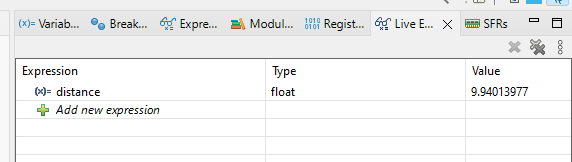
\includegraphics[width=.9\textwidth]{fig/element/dis10.png}
    \caption{Wynik dla odległości 10cm.}
    \label{fig:my_label}
\end{figure}

\vspace{1cm}

Zakres pomiarowy czujnika to 2 cm - 400 cm. Jak widać po odpowienim przeliczeniu danych jakie zwraca czujnik, otrzymujemy odległość w mm. Błąd pomiarowy, który występuje jest znikomy dlatego czujniki te bardzo dobrze sprawdzają się we wcześniej wspomnianych zastosowaniach.\\


Działanie czujnika zostało zaprezentowane na krótkim wideo. \cite{youtube}.
\clearpage
\newpage
\printbibliography[heading=bibintoc]

\end{document}
